\documentclass[journal]{IEEEtran}
\usepackage[T1]{fontenc}
\usepackage{amsmath,amssymb,amsthm,booktabs,array,tabularx,url,graphicx,enumitem}
\usepackage[hidelinks]{hyperref}
\usepackage{microtype}
\newcommand{\FPR}{\operatorname{FPR}}
\newcommand{\BA}{\operatorname{BA}}
\newcommand{\ind}{\mathbf{1}}
\newcommand{\ton}{TON-IoT}
\newcommand{\cic}{CICIoT2023}
\newcommand{\nb}{N-BaIoT}
\newtheorem{theorem}{Theorem}
\newtheorem{proposition}[theorem]{Proposition}
\newtheorem{definition}[theorem]{Definition}
\newtheorem{corollary}[theorem]{Corollary}
\hyphenation{data-set data-sets pre-pro-cess-ing}
\makeatletter
\newcommand{\tableinput}[1]{\@@input #1.tex }
\makeatother
% Automatically generated from independent raw-log recomputation.
\newcommand{\RFEnergy}{1206.787}
\newcommand{\RFFOne}{0.983864}
\newcommand{\RFRecallPct}{99.664}
\newcommand{\RFFPRPct}{1.538}
\newcommand{\RFFN}{57.8}
\newcommand{\RFFP}{504.5}
\newcommand{\RFBatchMS}{32.595}
\newcommand{\TQEnergy}{1193.719}
\newcommand{\TQFOne}{0.970439}
\newcommand{\TQRecallPct}{96.710}
\newcommand{\TQFPRPct}{1.364}
\newcommand{\TQFN}{565.9}
\newcommand{\TQFP}{447.5}
\newcommand{\TQBatchMS}{1.447}
\newcommand{\TQSavingJ}{13.068}
\newcommand{\TQSavingJLow}{9.736}
\newcommand{\TQSavingJHigh}{16.400}
\newcommand{\TQSavingPct}{1.082}
\newcommand{\TQFOneDropPP}{1.343}
\newcommand{\TQRecallDropPP}{2.954}
\newcommand{\DQEnergy}{1200.560}
\newcommand{\DQFOne}{0.970439}
\newcommand{\DQRecallPct}{96.710}
\newcommand{\DQFPRPct}{1.364}
\newcommand{\DQFN}{565.9}
\newcommand{\DQFP}{447.5}
\newcommand{\DQBatchMS}{1.482}
\newcommand{\DQSavingJ}{6.227}
\newcommand{\DQSavingJLow}{1.600}
\newcommand{\DQSavingJHigh}{10.853}
\newcommand{\DQSavingPct}{0.515}
\newcommand{\DQFOneDropPP}{1.343}
\newcommand{\DQRecallDropPP}{2.954}
\newcommand{\CFEnergy}{1196.842}
\newcommand{\CFFOne}{0.636440}
\newcommand{\CFRecallPct}{99.335}
\newcommand{\CFFPRPct}{59.164}
\newcommand{\CFFN}{114.4}
\newcommand{\CFFP}{19405.9}
\newcommand{\CFBatchMS}{2.337}
\newcommand{\CFSavingJ}{9.945}
\newcommand{\CFSavingJLow}{7.117}
\newcommand{\CFSavingJHigh}{12.773}
\newcommand{\CFSavingPct}{0.824}
\newcommand{\CFFOneDropPP}{34.742}
\newcommand{\CFRecallDropPP}{0.329}

\begin{document}
\title{When Learned IDS Model Selection Collapses to a Static Choice:\\A Measurement Study at the Edge}
\author{Nuonan~Ouyang,
        Adrian~Shatte,
        Zhigang~Lu,
        Chao~Chen,~\IEEEmembership{Member,~IEEE,}
        and~Wei~Xiang,~\IEEEmembership{Senior Member,~IEEE}%
\thanks{(\textit{Corresponding author: Nuonan Ouyang.})}%
\thanks{N. Ouyang and A. Shatte are with the College of Science and Engineering, Division of Research, James Cook University, Bebegu Yumba Campus, Building 17, Douglas, Townsville, QLD, Australia (e-mail: nuonan.ouyang@my.jcu.edu.au; adrian.shatte@jcu.edu.au; ORCID: 0009-0004-7124-8940; 0000-0002-6225-9697).}%
\thanks{Z. Lu is with the School of Computer, Data and Mathematical Sciences, Western Sydney University, Penrith (Kingswood) Campus, Kingswood, NSW, Australia (e-mail: z.lu@westernsydney.edu.au; ORCID: 0000-0001-5102-6217).}%
\thanks{C. Chen is with the College of Business and Law, RMIT University, Melbourne, VIC 3000, Australia (e-mail: chao.chen@rmit.edu.au; ORCID: 0000-0003-1355-3870).}%
\thanks{W. Xiang is with the Australian Centre for AI in Medical Innovation and the Cisco-La Trobe Centre for AI and Internet of Things, La Trobe University, Melbourne, VIC, Australia (e-mail: w.xiang@latrobe.edu.au; ORCID: 0000-0002-0608-065X).}%
}
\markboth{IEEE Transactions on Network and Service Management,~Vol.~XX, No.~XX, Month~Year}%
{Ouyang \MakeLowercase{\textit{et al.}}: When Learned IDS Model Selection Collapses to a Static Choice}
\maketitle
\begin{abstract}
Runtime model selection trades detection quality against energy and latency, but comparison only with a costlier static detector conflates detector choice with adaptive value. We present an analytic and physical measurement framework combining a pairwise reward criterion, matched static controls, paired blocks, a frozen load--prevalence factorial, and off-support action reporting. On one Raspberry Pi 4B with four frozen TON-IoT detectors, tabular Q-learning and DQN realize a static LightLR schedule. A retrospective validation-only audit excludes MedRF/LightLR and HeavyMLP/LightLR preference reversals but identifies seven TinyDT-favouring windows among 2,500; it does not prove global LightLR optimality. Under a $50/100/4000\text{ rows/s}\times0.10/0.50/0.90$ factorial, a causal DeadlineGuard saves 43.7~J per 500-s run against Static-MedRF (2.98\%; 95\% paired CI 41.4--46.0~J) and eliminates 512/5,000 deadline misses at a 1.373-percentage-point F1 cost. Off training support, Tabular-Q's deterministic tie rule selects TinyDT and reaches 67.76\% false-positive rate. These single-board results motivate joint auditing of reward attainability, realized actions, matched-static attribution, service feasibility, and off-support defaults.
\end{abstract}
\begin{IEEEkeywords}
Intrusion detection, IoT, edge resource management, model selection, reinforcement learning, service management, energy measurement, reproducibility.
\end{IEEEkeywords}
\section{Introduction}
Edge intrusion detection must trade security against latency and energy on tightly constrained hardware~\cite{Zhang2024VehicleEdge,Murti2024vRAN,Zhang2024DVFO}. Runtime model selection appears attractive, but a learned controller may simply choose one cheap detector. Comparing it only with a costlier static detector then attributes an operating-point change to adaptation. Reward normalization can create the same problem before training by making action reversal unattainable, while sparse discrete states can hide an unsafe default action until the workload moves off support.

We address these risks with an analytic and measurement framework. First, a pairwise non-degeneracy criterion decides from the declared reward, cost profile, and validation support whether two actions can ever exchange rank. Second, a five-instrument protocol requires trace-matched physical blocks, the static action actually realized by the selector, a prospectively frozen factorial, joint raw/drift-adjusted endpoints, and full on-/off-support action reporting. Third, we apply the framework on one Raspberry Pi 4B with four frozen TON-IoT detectors, Tabular-Q, DQN, a fixed confidence cascade, and a causal DeadlineGuard rule. Under the frozen $50/100/4000\text{ rows/s}\times0.10/0.50/0.90$ factorial, DeadlineGuard saves 43.7~J per 500-s run against Static-MedRF (2.98\%; 95\% paired CI 41.4--46.0~J) and eliminates all 512/5{,}000 deadline misses at a 1.373-pp F1 cost. The learned selectors instead realize LightLR on observed support; off support, Tabular-Q's deterministic tie rule selects TinyDT and yields 67.76\% FPR.

Four questions organize the study: \textbf{RQ1}, what security/resource operating points anchor the frozen detector pool? \textbf{RQ2}, do learned selectors beat the static schedule they realize, and does their reward admit preference reversal? \textbf{RQ3}, do confidence- and deadline-aware controls switch usefully under fixed and variable load? \textbf{RQ4}, how do state coverage, deadline violations, and validation-only threshold calibration constrain deployment claims? Our contribution is not a new RL algorithm; it is a reproducible service-management method that separates detector choice, conditional adaptation, objective design, and off-support safety. Figure~\ref{fig:experimentdesign} summarizes the physical apparatus and evidence path.

\begin{figure*}[t]
\centering
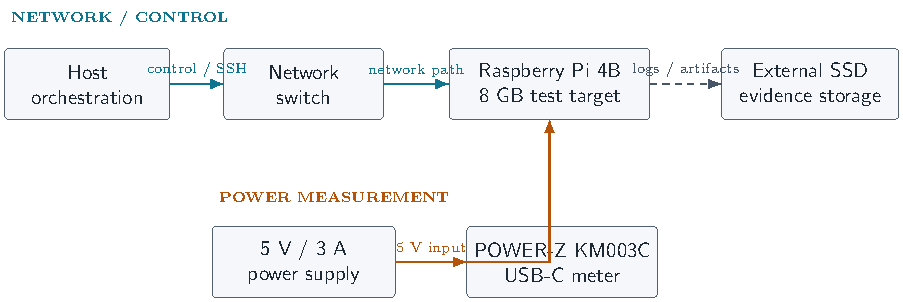
\includegraphics[width=.78\textwidth]{figures/experiment_setup_schematic.pdf}
\caption{Schematic apparatus overview. A 5-V supply feeds the Raspberry Pi 4B through the POWER-Z KM003C USB-C meter; network orchestration reaches the Pi via the switch; the external SSD stores evidence artifacts. The drawing shows roles and paths only.}
\label{fig:experimentdesign}
\end{figure*}

\section{Related Work}
\label{sec:relwork}
Our work sits at the intersection of edge IDS, conditional inference, model serving, and learned resource orchestration. Recent IDS research covers continual detection, heterogeneous representations, and runtime model selection~\cite{Wang2024BFSNID,AOCIDS2024,StatAvg2025,DMIDS2025}. Auto-IDaS and FEDMS show that learned or confidence-driven detector selection is operationally plausible~\cite{Lin2024AutoIDaS,Hasan2026FEDMS}, but neither a complex controller nor a cheaper operating point by itself establishes adaptive value. We therefore require comparison with the static detector actually realized by the selector and expose the full state--action map, not only visited-state occupancy.

Conditional-computation systems---including BranchyNet, adaptive network selection, MSDNet, and shallow--deep networks---escalate uncertain inputs to costlier models~\cite{Teerapittayanon2016BranchyNet,Bolukbasi2017Adaptive,Huang2018MSDNet,Kaya2019ShallowDeep}. Our fixed confidence cascade translates that idea to whole-device IDS measurement. It also exposes a serving detail often hidden by row-level escalation rates: only 1.34\% of rows escalate, yet they activate MedRF in 66.76\% of windows, so call granularity rather than row fraction governs the observed cost.

Serving systems such as Clipper, INFaaS, and Clockwork make accuracy, latency, and cost SLOs explicit and route requests among model variants~\cite{Crankshaw2017Clipper,Romero2021INFaaS,Gujarati2020Clockwork}. We adopt their service-contract perspective but add two missing controls: a matched static action that separates routing value from model choice, and a pre-deployment audit that asks whether the declared reward permits any action reversal on validation support.

RL-based edge orchestration spans vRAN, vehicle--edge scheduling, DVFS, offloading, and QoS control~\cite{Murti2024vRAN,Zhang2024VehicleEdge,Zhang2024DVFO,Lou2024Startup,Kim2024DistributedOffload,Maleki2024QCS,Nan2026RobustDNN,Wang2025TrustOffload,Hu2025SITOff}. Tabular Q-learning and DQN are representative discrete and neural value-based controllers~\cite{Watkins1992,Mnih2015}. Our contribution is not a new RL algorithm. It is a diagnostic methodology that combines an analytic reward screen, matched physical attribution, a prospectively frozen load/prevalence factorial with an explicit deadline SLO, and off-support action auditing. These instruments address known evaluation fragility in security ML and small-sample RL studies~\cite{Arp2022,Agarwal2021}.

\section{Compact System Model and Service Objectives}
\label{sec:system}
An edge node processes batches in decision windows $t=1,2,\ldots$ using a resident detector pool $\mathcal M=\{m_1,\ldots,m_K\}$. Before inference, a frozen controller commits one action $a_t=\pi(s_t)\in\mathcal M$ from the causal state
\begin{equation}\label{eq:state}
s_t=(\widetilde T_t,h_{t-1},q_t,\lambda_{t-1},a_{t-1}),
\end{equation}
where $\widetilde T_t$ is smoothed temperature, $h_{t-1}$ the preceding selected detector's mean posterior, $q_t$ queue utilization, $\lambda_{t-1}$ preceding arrival count, and $a_{t-1}$ preceding action. Ground truth, current outputs of unselected detectors, and factorial-cell identity are unavailable at decision time. Because all models remain resident, selection excludes fitting and model-loading cost.

For each completed window we record attack-class F1, recall, and false-positive rate; completion latency is checked against deadline $\Delta_{\rm SLO}$; and resource cost is whole-device USB energy. In the physical study $\Delta_{\rm SLO}=1$~s and each run lasts 500~s. Training optimizes a scalar surrogate, but evaluation jointly reports security, timeliness, energy, action occupancy, and state support. Test policies are frozen and never updated online.

The network-layer adversary may vary traffic prevalence and arrival rate but cannot alter the meter, controller memory, detector artifacts, or training pipeline. Adversarial-ML attacks and hardware tampering are outside scope. The operational risk considered here is induced entry into unvisited discrete states: deterministic ties can then expose an unaudited default action.

We credit a selector with \emph{adaptive value} only when it realizes more than one action on deployment support, improves a service objective without a comparable regression, and survives a paired comparison with the static instance of its dominant realized action. Otherwise the measured difference is attributed to detector operating-point choice rather than conditional adaptation.

\section{Dataset-Native Data Preparation}
\label{sec:data}
\subsection{Choice of Primary Dataset}
The primary systems study uses TON-IoT~\cite{TONSource}. Its records combine IoT service telemetry, operating-system events, and networked interactions labeled with attack categories, making the dataset representative of the mixed-signal traffic that reaches an edge IDS at the service boundary rather than at the wire only. We deliberately restrict the physical dynamic-power study to a single dataset because coupling multiple encoded pipelines to one hardware campaign would confound feature dimensionality, class balance, and physical measurement; instead \cic{}~\cite{CICSource} and \nb{}~\cite{NBaIoTSource} are retained as supplementary detector and coverage audits and are not used to imply cross-dataset dynamic-power generalization.

\subsection{Frozen Preprocessing and Splits}
The TON-IoT pipeline is frozen and retains 32 native features. Imputation, scaling, and categorical encoding are fitted on training data only and applied deterministically to validation and test. The split groups unordered IP pairs so that traffic patterns are not divided across partitions; the grouping rule hashes ``$11\vert$'' concatenated with the sorted IP pair and thresholds the first sixteen SHA-256 hexadecimal digits modulo 100 (training below 60, validation 60--79, test 80--99). Training seed 11 fixes all model fits, so any single-seed conclusion is explicit rather than implied. Source-row identifiers and raw-field-string fingerprints are cross-partition disjoint, and an independent encoded-float32 audit finds \emph{zero} TON-IoT train--test vector matches, which addresses a commonly-cited leakage risk in IoT IDS benchmarks~\cite{Arp2022}.

\subsection{Auxiliary Dataset Audits}
The same ledger retains dataset-native \cic{} and \nb{} pipelines with 39 and 115 native features respectively. For \cic{}, seventeen attack labels remain training-only because their capture files are too few for a defensible test split; the actual test taxonomy is a binary attack-versus-normal partition over sixteen attack categories plus benign traffic. For \nb{}, physical device identifiers are the grouping unit, giving five training, two validation, and two test devices; a post-hoc byte-level audit records that 17.3\% of \nb{} test rows share exact float32 vectors with training rows (seven distinct vectors), reflecting the sensor-repetition structure of the dataset rather than a preprocessing fault. These coverage and encoded-overlap limitations are retained rather than used to imply cross-dataset dynamic-power generality; consequently the auxiliary datasets support only static classification and replay evidence.

\subsection{Class Balance and Replay Traces}
The TON-IoT test set contains a majority attack fraction, which is common in IoT benchmarks and which we do not rebalance because the physical study measures whole-device behavior on the natural distribution. To probe operating points under controlled prevalence shifts, the supplement retains twenty static replay traces per model (fifty per dataset before deduplication), with successive phase attack fractions $\{0.05, 0.35, 0.70, 0.40, 0.10\}$ over $\{100, 100, 120, 100, 80\}$ windows. These traces do not constitute a new detector-training exercise; they resample fixed held-out pools to expose how a frozen detector's F1 and balanced accuracy behave when prevalence, not distribution, changes.

\section{Detector Pool, Reward Specification, and Non-degeneracy Framework}
\label{sec:methods}
This section specifies the frozen detector artifacts, the reward specification used by both learned controllers, and the pre-deployment pairwise non-degeneracy screening test. The last of these is stated as a theorem so that it can be applied to future learned selectors without re-derivation.

\subsection{Detector Pool}
Each dataset has four separately fitted configurations: depth-6 TinyDT; L2-regularized LightLR; 25-tree, depth-10 MedRF; and a 64/32/16 HeavyMLP. All use threshold 0.5 and training seed 11. Detector names do not assert a resource ranking; the physical measurements determine the empirical order. During TON-IoT physical experiments all models remain resident, and an action selects one model for the next batch without loading, fitting, or updating it. This design deliberately isolates the effect of controller decisions from model instantiation cost so that any observed switching cost is attributable to inference itself, not to hot-swapping detectors.

\subsection{Causal State Encoding}
Before window $t$ the controller constructs $s_t$ per~\eqref{eq:state}. The kernel temperature is smoothed as $\widetilde T_t=0.9\widetilde T_{t-1}+0.1T_t$, initialized at $T_0$. The threat observation $h_{t-1}$ is the arithmetic mean attack probability from the single detector selected in the preceding window; it is \emph{not} the preceding ground-truth attack fraction. Queue utilization is bounded to $[0,1]$, and the preceding arrival count is divided by 100 and bounded to $[0,2]$. Initial values are $h_0=0.5$, $\lambda_0/100=1$, and $a_0=\text{TinyDT}$.

Each of the first four state variables has three bins. Their two boundaries are $(45,70)$~$^{\circ}$C, $(1/3,0.7)$ for threat, $(1/3,2/3)$ for queue utilization, and $(0.9,1.1)$ for arrival ratio. Including four previous actions yields $3^4\times 4=324$ encoded states. Boundary equality enters the higher bin. The flat index is row-major in the listed order, with previous action changing fastest.

The executed order within a window is: (i) state construction from causal telemetry and lagged context; (ii) action commitment and log; (iii) selected-detector inference; (iv) outcome log; and (v) lagged-state update for $t+1$. Ground truth, cell identity, and unselected current-window outputs are unavailable online. This information boundary is what enables preference-reversal analysis to be conducted purely on state features that the deployment can observe.

\subsection{Reward and Cost Provenance}
The unchanged per-window training reward is
\begin{equation}\label{eq:reward}
    r_t = 0.5\,B_t \;-\; 0.2\,\overline P_t \;-\; 0.2\,\overline L_t \;-\; 0.1\,\overline H_t,
\end{equation}
where $B_t$ is balanced accuracy over the classes present in the window. With $[x]_0^1=\min(1,\max(0,x))$, the normalization is
\begin{align}
    \overline P_t &= \left[\tfrac{P_t-2.347219336}{0.049806200}\right]_0^1, & \overline L_t &= \left[\tfrac{L_t-1.2979595}{29.6547998}\right]_0^1,\\
    \overline H_t &= \left[\tfrac{\max(0,T_t^{\rm post}-\widetilde T_t)}{1\,^{\circ}\mathrm{C}}\right]_0^1.
\end{align}
$P_t$ and $L_t$ are frozen TON-IoT paced-profile lookups, not contemporaneous training measurements. Their means, listed as (power W, batch latency ms) for the four detectors, are 2.353132/1.297960 for TinyDT, 2.347219/1.544420 for LightLR, 2.397026/30.952759 for MedRF, and 2.366688/4.417836 for HeavyMLP. The compact software traces contain no post-action temperature response: their adapter supplies a fixed 35$^{\circ}$C predecision value and reuses that action-invariant value in the outcome field. Thus $\overline H_t=0$ throughout the executed training and validation traces; it is not an action-level thermal cost. No fitted thermal response or switching-energy penalty is used, and consequently no thermal control action is claimed.

\subsection{Pairwise Non-degeneracy Criterion}
Reward normalization is often reported as a hyperparameter without evidence that it permits any state to reverse the preferred action. We now show that this question can be answered before deployment with only the declared weights, cost profile, and a support region.

Consider two actions $a,b\in\mathcal M$. Decompose the scalar utility into a detection contribution and a normalized resource cost:
\begin{equation}
    U_a(s) = w_D\, D_a(s) - C_a,\qquad C_a=\sum_j w_j\,\overline C_{j,a},
\end{equation}
where $w_D=0.5$ in our specification and $\overline C_{j,a}$ collects the normalized resource penalties that are fixed on the declared support (as they are for the executed paced profiles at neutral thermal cost). Let $\Delta D_{ab}(s)=D_a(s)-D_b(s)$ and $\Delta C_{ab}=C_a-C_b$. Then
\begin{equation}\label{eq:diff}
    U_a(s)-U_b(s) = w_D\,\Delta D_{ab}(s) - \Delta C_{ab},\qquad
    \tau_{ab}=\frac{\Delta C_{ab}}{w_D}.
\end{equation}

\begin{theorem}[Pairwise non-degeneracy]\label{thm:nondeg}
Let $\mathcal S$ be a support region. Under the frozen scalar utility~\eqref{eq:diff}, a strict pairwise preference reversal between actions $a$ and $b$ exists on $\mathcal S$ if and only if
\begin{equation}\label{eq:nondeg}
    \min_{s\in\mathcal S}\Delta D_{ab}(s) < \tau_{ab} < \max_{s\in\mathcal S}\Delta D_{ab}(s).
\end{equation}
If \eqref{eq:nondeg} fails, every $s\in\mathcal S$ yields the same sign of $U_a(s)-U_b(s)$; consequently no policy that maximizes the frozen utility can prefer $a$ on one state and $b$ on another within $\mathcal S$.
\end{theorem}

\begin{corollary}[Attainability under bounded detection]\label{cor:bound}
If $D_a(s),D_b(s)\in[0,1]$ for every $s\in\mathcal S$, then reversal is impossible whenever $|\tau_{ab}|\ge 1$; and reversal is guaranteed impossible whenever the attainable interval $[\min\Delta D_{ab},\max\Delta D_{ab}]$ does not straddle $\tau_{ab}$.
\end{corollary}

Because balanced accuracy lies in $[0,1]$, the corollary gives an immediate ceiling. Under the executed candidate-range scaling, the frozen nonthermal penalties imply $\tau_{\text{MedRF},\text{LightLR}}=0.7967$. A reproducible audit of all 2{,}500 windows in the five hash-bound validation traces finds $\Delta D_{\text{MedRF},\text{LightLR}}\in[-0.1053,0.1053]$, so this threshold lies outside the observed validation-window support. This retrospective audit excludes MedRF/LightLR and HeavyMLP/LightLR reversal on observed validation support. TinyDT/LightLR can reverse: TinyDT has higher immediate reward in 7 of 2{,}500 validation windows. These label-informed window comparisons establish neither optimality over all encoded states nor optimal long-horizon return, and do not fully explain the learned collapse. There is no evidence that this audit preceded test inspection. Supplementary Theorem~S1 gives the proof, Supplementary Table~S11A gives the full pairwise matrix, and Supplementary Algorithm~S1 gives the validation-only reward audit. If reversal is unattainable, the engineer should use an audited static schedule or renormalize against an external deployment contract---for example idle-relative power, the latency SLO, an energy envelope, or thermal headroom---rather than against detector-pool extrema.

\subsection{Policies}
Four policies are evaluated in the physical study. \emph{Static-\{TinyDT, LightLR, MedRF, HeavyMLP\}} freeze a single detector. \emph{CFSM} is a fixed heuristic initialized to TinyDT; at a smoothed temperature of at least 70~$^{\circ}$C it steps down one model rank, bypassing cooldown; otherwise it holds for two windows after a switch and steps down/up one rank when threat crosses 0.7. Queue and load are logged but not used by CFSM. \emph{Tabular-Q} uses zero initialization, $\alpha=0.1$, $\gamma=0.9$, and the update
\begin{equation}
    \begin{aligned}
        Q(s_t,a_t) &\leftarrow Q(s_t,a_t) + 0.1\,\delta_t,\\
        \delta_t &= r_t + 0.9\max_a Q(s_{t+1},a) - Q(s_t,a_t),
    \end{aligned}
\end{equation}
with zero terminal bootstrap~\cite{Watkins1992}. \emph{DQN} uses one-hot state, two 64-unit ReLU layers, Adam $10^{-3}$, replay 10{,}000, batch 32, and a target copy every 250 updates~\cite{Mnih2015}. Both learners train for 1{,}000 episodes with $\varepsilon$ linearly annealed from 1 to 0.01; checkpoints are selected every 25 episodes on five validation traces. Test execution freezes the policy and performs no update.

Two prospectively frozen causal policies join the reviewer campaigns. \emph{ConfidenceCascade} first executes LightLR on the full 100-row batch and, when its posterior $p_{\text{LR}}$ falls in $[0.3,0.7]$, invokes MedRF once on the deferred sub-batch. \emph{DeadlineGuard} uses only the current causal arrival count $N$: it selects MedRF when the predicted MedRF cost $\lceil N/100\rceil L_{95}^{\text{RF}}\le 1$~s, otherwise LightLR. Both thresholds were frozen from pre-experiment latency data.

Archived process-start and policy-creation timestamps indicate approximately 26.7~s for the Tabular-Q training run and 256.9~s for DQN; these are provenance-derived wall-clock intervals rather than calibrated compute benchmarks, and training energy was not instrumented. Deployment cost is measured separately in Section~\ref{sec:dynamicresults}.

The runtime sequence is causal: observe telemetry and lagged context; encode $s_t$; commit and log $a_t$; run only the selected resident detector; log outcome and telemetry; then update the lagged state. Ground truth is used only after the outcome during offline training. Formal test deployment freezes the policy and omits the update.

\section{Evaluation Protocol and Measurement Instrumentation}
\label{sec:eval}
Our evaluation protocol is designed to separate detector choice from adaptive value along five instruments: (i) paired physical blocks across trace-matched detectors; (ii) matched-static-action attribution controls; (iii) prospectively frozen factorial workloads; (iv) separate raw and drift-adjusted power endpoints; and (v) full occupancy and off-support action reporting. This section describes each instrument together with the classification, timing, and power measurement pipelines that feed them.

\subsection{Classification and Static Evidence}
The held-out classification evaluation uses the frozen threshold 0.5 and reports attack-class F1, recall, balanced accuracy, false-positive rate, and the full confusion counts. In particular,
\begin{align}
    \FPR &= \frac{FP}{TN+FP},\qquad F1 = \frac{2TP}{2TP+FP+FN},\\
    \BA &= \tfrac12\!\left(\tfrac{TP}{TP+FN}+\tfrac{TN}{TN+FP}\right).
\end{align}
Counts are pooled over the declared evaluation unit before metrics are calculated. The supplement retains 50 static traces and 200 model--trace evaluations; these reuse fixed held-out pools and do not constitute fresh attacks, classifier retraining, or physical repeats.

\subsection{Pi Prediction Consistency and Inference Timing}
Pi parity checks cover 12 dataset--model combinations and 10{,}000 encoded rows each with \emph{zero} threshold-label disagreements against the training-host outputs. Tight-loop timing reports 100-row inference after warm-up and excludes encoding, transport, queueing, and controller cost; these boundaries are re-stated wherever a timing figure is used.

\subsection{Static Whole-Device Power}
The physical reference uses one Raspberry Pi 4B 8~GB and an inline POWER-Z KM003C USB-C meter. Fifteen valid 1{,}800-second segments comprise three repeats of instrumented idle and four TON-IoT detectors, all resident, at 100 pre-encoded rows/s. This is resource characterization, not another detection test.

The meter records nominally 1~Hz boundary samples, including raw ADC replies, signed current, voltage, and monotonic request/receive times. Under the recorded connector orientation, consumed power is $P_i=V_i(-I_i)$. Using the observed sampling times $\tau_i$, input energy is approximated by
\begin{equation}\label{eq:trap}
    E=\sum_{i=1}^{n-1}\frac{P_i+P_{i+1}}{2}(\tau_{i+1}-\tau_i),\qquad
    \bar P = \frac{E}{\tau_n-\tau_1}.
\end{equation}
No missing sample is filled. This is 1-Hz load-side USB energy, not calibrated wall-side measurement or a subsecond waveform.

\subsection{Statistical Units and Interval Reporting}
For an outcome $z$ observed over $n$ declared repetitions, the two-sided Student-$t$ interval is
\begin{equation}\label{eq:tci}
    \bar z\pm t_{0.975,\,n-1}\,\frac{s_z}{\sqrt n},
\end{equation}
using the sample SD~\cite{NISTMean}. Physical scheduler inference uses \emph{ten paired blocks}, never rows, windows, or meter frames. Raw energy is primary. Drift sensitivity subtracts each run's immediately preceding idle power; it is reported separately rather than substituted for raw measurement. Exact $2^{10}$ sign-flip tests supply a non-parametric robustness diagnostic under sign-symmetry and exchangeability, and are reported alongside the classical interval when both directional stability and magnitude precision matter.

\subsection{Physical Campaigns Overview}
Six physical campaigns are executed. The \emph{primary} campaign contains ten matched 500-second blocks of Static-MedRF, CFSM, Tabular-Q, and DQN. \emph{P1A} adds ten matched blocks with Static-LightLR to enable the attribution comparison against the static action the learned policies realize. \emph{P1B} isolates state-to-action decision timing. \emph{P1C--P1E} test seed, reward/state, and Tabular-Q $\alpha/\gamma$ variations. \emph{R1} adds ten matched blocks at 100 rows/s comparing Static-LightLR, the confidence cascade, frozen Tabular-Q, and Static-MedRF. \emph{R2} adds ten matched blocks and six methods over a prospectively frozen $50/100/4000\text{ rows/s}\times 0.10/0.50/0.90$ prevalence factorial with a fixed one-second service deadline. Two additional protocols are recorded: \emph{R3} was predeclared for controller-only power measurement but stopped before execution because its four-state design condition became ambiguous once the frozen artifact was inspected; \emph{R4} is a post-hoc TinyDT threshold diagnostic conducted on validation only. R3 and R4 are reported in full because omitting either would misrepresent the executed evaluation surface.

\section{Static and Attribution Results}
\label{sec:staticresults}
This section reports the classification operating points, the static physical resource characterization, and the primary/P1A attribution and robustness evidence. Together these anchor the pairwise non-degeneracy analysis of Section~\ref{sec:methods} in measured, rather than declared, cost profiles.

\subsection{TON-IoT Detection Operating Points}
Table~\ref{tab:classification} shows the four TON-IoT operating points used by the physical study. TinyDT has recall 0.9976 but F1 0.4792 and FPR 67.78\%; LightLR, MedRF, and HeavyMLP have F1 0.9620--0.9746 and FPR 1.35--1.52\%. MedRF's aggregate held-out balanced-accuracy advantage over LightLR is 0.0140; this post-freeze test statistic is descriptive and is not treated as a statewise attainability bound. The non-degeneracy conclusion instead uses the validation-only window audit in Section~\ref{sec:methods}, where the observed difference range $[-0.1053,0.1053]$ does not straddle $\tau_{\text{MedRF,LightLR}}=0.7967$. Full confusion counts, plus \cic{}/\nb{} detector and overlap audits, are retained in the supplement.

\begin{table}[t]
\centering\small
\caption{TON-IoT held-out detection at threshold 0.5. BA denotes balanced accuracy; FPR is a percentage.}
\label{tab:classification}
\setlength{\tabcolsep}{4.2pt}
\begin{tabular}{lrrrr}\toprule
Model & F1 & Recall & BA & FPR (\%)\\\midrule
\tableinput{tables/ton_classification_rows}
\bottomrule\end{tabular}
\end{table}

For attack prevalence $p$, recall $r$, and FPR $f$,
\begin{equation}\label{eq:prevalence}
    F1 = \frac{2pr}{p(1+r) + (1-p)f},
\end{equation}
so high attack prevalence can coexist with high F1 and poor normal-class behavior. This identity motivates our decision to report attack-class F1, recall, and FPR jointly throughout, rather than summarising with F1 alone.

\subsection{Static Physical Resource Measurements}
Across fifteen static segments, idle averages 2.335~W and active means span 2.347~W (LightLR) to 2.397~W (MedRF). MedRF's paired increment is 61.6~mW with 95\% CI $[32.1,\,91.0]$; TinyDT and LightLR intervals cross zero, indicating that the whole-device signal at this cadence is dominated by background platform power. No accepted workload window records undervoltage or throttling. Full segment statistics are supplementary; labels such as ``Tiny'' or ``Heavy'' are not used as empirical cost ranks.

\subsection{Primary Dynamic Comparison}
All forty primary runs contain 501 power samples and 500 decisions. Relative to Static-MedRF, Tabular-Q saves \TQSavingJ{} J (95\% paired CI \TQSavingJLow{}--\TQSavingJHigh{}) and DQN saves \DQSavingJ{} J (\DQSavingJLow{}--\DQSavingJHigh{}), but both lose \TQFOneDropPP{} F1 pp and \TQRecallDropPP{} recall pp. Both select LightLR in all 5{,}000 windows; consequently the primary contrast measures a detector operating-point change and not adaptive switching. This is the core observation that motivates the P1A attribution control below.

\subsection{P1A: Matched Attribution Against Static-LightLR}
P1A executes ten matched blocks comparing Tabular-Q, DQN, Static-LightLR, and Static-MedRF on the same traces. Because both learned policies realize LightLR throughout, Static-LightLR is the correct baseline for isolating adaptive value. Table~\ref{tab:p1a} reports the four key paired contrasts.

\begin{table}[t]
\centering\footnotesize
\caption{P1A paired contrasts, ten trace-matched blocks. $\Delta E$ is first-minus-second method; the sign-flip $p$ column is an exact non-parametric diagnostic over the ten block-level differences.}
\label{tab:p1a}
\setlength{\tabcolsep}{3.0pt}
\resizebox{\columnwidth}{!}{%
\begin{tabular}{lcrr}\toprule
Contrast & Outcome & Mean & 95\% CI\\\midrule
Tabular-Q $-$ Static-LightLR & Energy (J) & $+0.456$ & $[-1.861,+2.772]$\\
Tabular-Q $-$ Static-LightLR & Power (mW) & $+0.910$ & $[-3.722,+5.542]$\\
DQN $-$ Static-LightLR       & Energy (J) & $+4.525$ & $[+2.693,+6.357]$\\
DQN $-$ Static-LightLR       & Power (mW) & $+9.045$ & $[+5.381,+12.709]$\\
Static-MedRF $-$ Static-LightLR & Energy (J) & $+12.471$ & $[+10.611,+14.331]$\\
Static-MedRF $-$ Static-LightLR & F1 (pp)    & $+1.343$  & $[+1.292,+1.393]$\\\bottomrule
\end{tabular}}
\end{table}

Three findings emerge. First, Tabular-Q's energy contrast against the matched Static-LightLR control has an interval that includes zero, so the primary campaign's 13.1-J saving against Static-MedRF is fully explained by detector operating-point choice rather than by adaptation. Second, DQN carries a small but resolvable +4.5-J energy premium over Static-LightLR despite reproducing identical detection, indicating that its per-window controller cost, while a tiny fraction of the second, is not free at 100 rows/s. Third, Static-MedRF's +12.5-J energy penalty against Static-LightLR is closely matched by the primary Tabular-Q saving against Static-MedRF, which confirms the compositional picture: (Static-MedRF $-$ Static-LightLR) $\approx$ (Static-MedRF $-$ Tabular-Q).

\subsection{P1B: Isolated Scheduler Overhead}
The isolated benchmark reports state-to-action decision time on the observed state support after correction of an earlier benchmarking substitution that was retained as an invalid attempt in the archive. On observed support, means are 0.739~$\mu$s for Static-LightLR, 6.582~$\mu$s for CFSM, 10.796~$\mu$s for Tabular-Q, and 1.567~ms for DQN. DQN is roughly $145\times$ Tabular-Q's controller cost but remains 0.157\% of the one-second decision interval. These timings are not converted into joules; the R2 physical evidence in Section~\ref{sec:dynamicresults} bounds what can be attributed to controller cost alone.

The full 240-unit benchmark, confidence intervals, and raw timing arrays are retained in Supplementary Table~S15.

\subsection{P1C--P1E: Multi-seed and Sensitivity Coverage}
P1C trains ten additional Tabular-Q and ten additional DQN policies under the frozen state, reward, split, and training-horizon protocol. All twenty policies select LightLR in 100\% of held-out windows (Wilson 95\% interval $[0.7225, 1.0]$). Greedy full-state maps vary across seeds---for DQN especially, from 0/324 to 311/324 TinyDT cells---but the observed-support behavior is unanimous, evidence for policy stability that is scoped to that support rather than to the whole encoded grid.

P1D varies the reward weights and separately ablates each state component; all 85 valid policies are single-action on held-out support. Only the five \emph{detection-only} Tabular-Q variants---those with all resource penalties removed---switch the collapsed action away from LightLR to MedRF, describing these frozen runs rather than proving that resource-aware policies must choose LightLR. All thirty state-ablation policies remain single-action LightLR, indicating that no single state component was the mechanism suppressing switching. P1E adds 35 Tabular-Q runs across $\gamma\in\{0,0.5,0.9,0.99\}$ and $\alpha\in\{0.05,0.10,0.20\}$; all thirty-five collapse to LightLR.

The full P1C--P1E matrices are retained in Supplementary Tables~S16--S18. Together with Table~\ref{tab:p1a}, they document the observed collapse through matched attribution, isolated timing, and sanctioned reward/state/hyperparameter perturbations. Only removing all resource penalties changes the collapsed detector in this matrix; this is not a proof of global optimality.

\section{Dynamic Scheduler Results Under Fixed and Variable Load}
\label{sec:dynamicresults}
This section reports the two prospectively frozen reviewer campaigns and the two diagnostic protocols. R1 stresses a fixed-load confidence cascade; R2 stresses a load- and prevalence-varying factorial with an explicit one-second deadline SLO. R3 is a predeclared stop and R4 is a validation-only calibration diagnostic. Together they measure when conditional selection adds value and when it does not.

\subsection{R1: Fixed-Rate Confidence Cascade}
Table~\ref{tab:r1} reports ten new matched blocks at 100 rows/s. The fixed cascade escalates 1.34\% of rows and raises F1 by 1.347~pp over Static-LightLR while spending +7.952~J with 95\% CI $[5.897,\,10.007]$~J. Its raw mean-power difference is +15.917~mW $[11.798,\,20.035]$, whereas the preceding-idle adjustment gives +13.635~mW $[-1.515,\,28.784]$: environmental drift therefore weakens the power attribution but not the raw-energy result. Cascade F1 (0.98391) matches Static-MedRF (0.98386) within a few $10^{-5}$, at 0.279~pp lower recall and 0.156~pp lower FPR.

\begin{table*}[t]
\centering\footnotesize
\caption{R1 fixed-rate physical results; means over ten paired blocks. Adjusted power subtracts the immediately preceding idle. Escalation is the fraction sent from LightLR to MedRF.}
\label{tab:r1}
\setlength{\tabcolsep}{4.0pt}
\begin{tabular}{lrrrrrrr}\toprule
Method & Energy (J) & Power (W) & Adjusted (mW) & F1 & Recall (\%) & FPR (\%) & Escalation (\%)\\\midrule
\tableinput{tables/r1_revision_rows}
\bottomrule\end{tabular}
\end{table*}

\subsubsection*{Cascade cost is a call-granularity phenomenon, not a bound}
The apparently disproportionate cascade latency at a 1.34\% escalation rate is explained by call granularity. The frozen source performs \emph{one} MedRF call per escalation-active window on the deferred sub-batch, not one MedRF call per deferred row. Although only 1.3388\% of the 500{,}000 rows are deferred, they land in 3{,}338 of 5{,}000 windows (66.76\%), with a mean of only 2.01 deferred rows per active window. No-escalation windows average 1.636~ms; any-escalation windows average 31.884~ms, close to the cost of a single MedRF batch call regardless of sub-batch size; the overall mean is 21.830~ms. This is an operating-point description, not a general bound: an optimized batched cascade with wider windows or amortized MedRF calls would show a different profile. What the measurement establishes is that reporting only the escalation \emph{fraction} would be misleading; escalation \emph{prevalence across windows} is the operational cost driver.

\subsection{R2: Variable-Load Factorial and DeadlineGuard}
R2 is the campaign in which conditional selection can, in principle, demonstrate adaptive value: every 500-second run visits each of the nine load-by-prevalence cells exactly once, followed by a 50-second recovery cell. All controllers see causal telemetry only; no method sees the factorial cell identity. Table~\ref{tab:r2} reports the six-method means; Table~\ref{tab:r2pairs} lists the two paired contrasts we treat as headline endpoints.

\begin{table*}[t]
\centering\footnotesize
\caption{R2 variable-load results over ten paired blocks. Energy is mean$\pm$SD across runs; deadline miss is the fraction of one-second windows missing the service deadline; completion p95 is the 95th-percentile window completion latency.}
\label{tab:r2}
\setlength{\tabcolsep}{3.1pt}
\begin{tabular}{lrrrrrrr}\toprule
Method & Energy (J) & Power (W) & F1 & Recall (\%) & FPR (\%) & Miss (\%) & Completion p95 (s)\\\midrule
\tableinput{tables/r2_revision_rows}
\bottomrule\end{tabular}
\end{table*}

\begin{table}[t]
\centering\scriptsize
\caption{Headline R2 paired contrasts, $n=10$ blocks. $\Delta E$ is first-minus-second method; detection and deadline changes are percentage points.}
\label{tab:r2pairs}
\resizebox{\columnwidth}{!}{%
\begin{tabular}{lrrrr}\toprule
Contrast & $\Delta E$ (J), 95\% CI & $\Delta$F1 & $\Delta$Miss & sign-flip $p$\\\midrule
\tableinput{tables/r2_key_paired_rows}
\bottomrule\end{tabular}}
\end{table}

\subsubsection*{DeadlineGuard: causal switching adds measurable value}
DeadlineGuard executes MedRF in 3{,}500 and LightLR in 1{,}500 of its 5{,}000 windows and records a mean 5.3 switches per run. Against Static-MedRF, it uses 43.714~J less per run (95\% paired CI 41.418--46.010~J), a 2.98\% reduction relative to the 1{,}468.1-J Static-MedRF mean, while cutting the deadline-miss rate by 10.24~pp to zero. The trade-off is 1.373~pp lower F1 and 2.853~pp lower recall. All ten energy differences share sign (exact sign-flip $p=0.00195$). This is the campaign's positive result: a simple causal rule with a single binary observable achieves measurable energy savings and eliminates the SLO violations under variable load, an outcome that neither learned selector reproduces.

Against Static-LightLR, DeadlineGuard trades +7.550~J $[5.033,\,10.068]$ for a +0.06-pp F1 gain and preserves zero deadline misses. This second contrast is deliberately less dramatic: Static-LightLR is already feasible under the deadline SLO at 4{,}000 rows/s because its inference is fast; DeadlineGuard buys back a small detection-quality gap by escalating to MedRF only where that gap matters. The comparison of the two contrasts is the design lesson: DeadlineGuard is not universally optimal; it is optimal against the high-security static baseline that becomes infeasible at the deadline, and moderate against the low-security static baseline that remains feasible.

\subsubsection*{The learned selectors fail to adapt under variable load}
Frozen DQN remains LightLR in all 5{,}000 windows and reproduces the LightLR detection endpoints. Frozen Tabular-Q, in contrast, reaches new load-related states never visited during training; the zero-initialized Q rows are tied, \texttt{np.argmax} returns the first maximum, and TinyDT is action index zero. The registry labels this ``fallback'' but the frozen source contains no separate exception branch: the R2 outcome is the hardware realization of the off-support tie behavior already visible in the 314/324-state TinyDT greedy map of the primary Q table. The resulting run-level F1 is 0.7434 and FPR is 67.76\%. This is a directly transferable safety risk of sparse discrete controllers whose default action ordering is not itself audited.

\subsubsection*{Heterogeneous variance and preceding-idle drift}
R2 raw energy is heterogeneous across methods. For DQN versus Static-LightLR, all ten raw block differences are positive (median +5.72~J; exact sign-flip $p=0.00195$), but a single Block-4 excursion is +392.0~J. That block's preceding idle is 3.919~W with a 49.2~$^{\circ}$C maximum temperature, unlike the other DQN blocks. The excursion inflates the SD of paired differences to 122.2~J and expands the Student-$t$ interval to $[-43.2,\,131.7]$~J. Preceding-idle adjustment does not resolve the DQN--LightLR contrast. We therefore retain both the consistent raw direction and the unstable magnitude and \emph{do not} claim a controller-power attribution, because R3 was not executed. This is exactly the sort of finding for which our protocol requires raw and drift-adjusted endpoints to be reported side by side. Figure~\ref{fig:r2dashboard} combines the corresponding occupancy, deadline, support, and security diagnostics.

\begin{figure*}[!t]
\centering
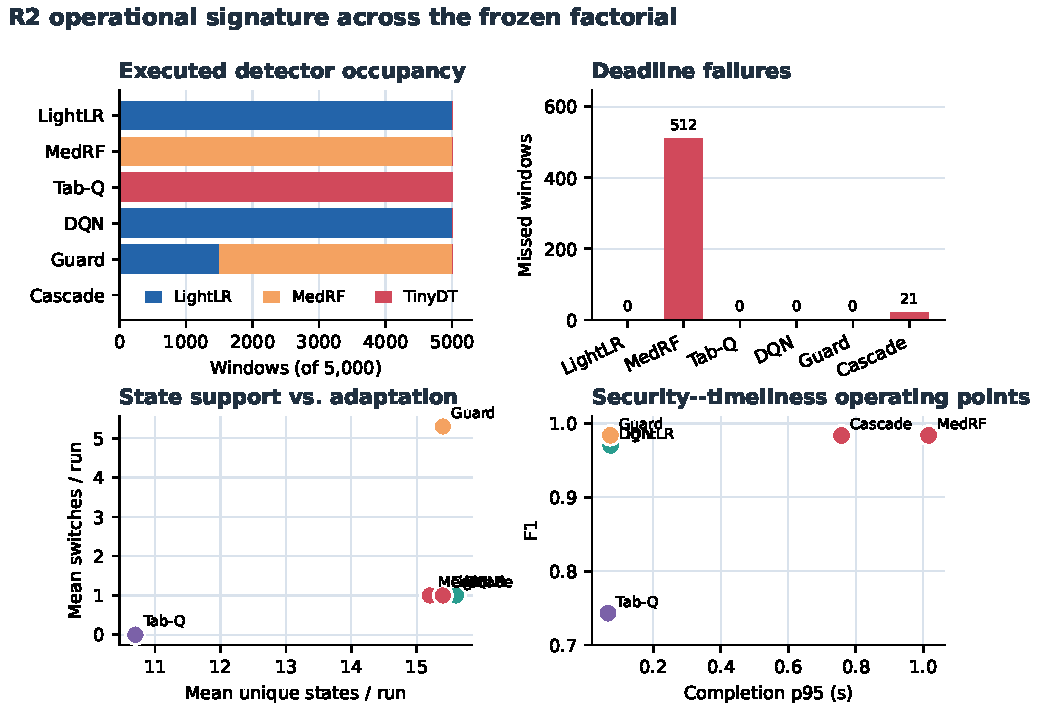
\includegraphics[width=.94\textwidth]{figures/r2_operational_dashboard.pdf}
\caption{R2 operational dashboard: realized detector occupancy, deadline misses, state support and switching, and security--timeliness operating points across the frozen 60-run factorial. DeadlineGuard is the single method with true load-conditioned switching and zero deadline misses; Tabular-Q's TinyDT collapse under new load states is visible in the occupancy panel.}
\label{fig:r2dashboard}
\end{figure*}

\subsection{R3: Protocol-Preserving Stop}
R3 predeclared controller-only physical power over four ``original observed-support states'' for isolated attribution. The frozen artifact exposes eight such states and supplies no outcome-independent rule for selecting four. Choosing four \emph{after the fact} would allow controller-power reporting to be driven by known R2 results, so the campaign stopped before measurement per the predeclared stop rule. No controller-only joule value is claimed. Reporting the stop rather than filling it silently preserves the integrity of the pairwise DQN--LightLR contrast above, which is why the DQN R2 magnitude is deliberately left as unresolved.

\subsection{R4: Threshold Calibration Diagnostic}
R4 selects a TinyDT threshold on validation by maximum balanced accuracy (highest-threshold tie-break), hashes it, and applies it \emph{once} to test. Table~\ref{tab:r4} contrasts the frozen primary threshold with the validation-selected diagnostic.

\begin{table}[t]
\centering\scriptsize
\caption{TON-IoT TinyDT test: fixed primary versus post-hoc validation-selected threshold. The diagnostic does not replace the primary threshold; it isolates calibration sensitivity as an explanation for the primary failure.}
\label{tab:r4}
\setlength{\tabcolsep}{2.1pt}
\resizebox{\columnwidth}{!}{%
\begin{tabular}{lrrrrrrrrr}\toprule
Result & $\tau$ & TN & FP & FN & TP & F1 & Rec. & FPR & BA\\\midrule
\tableinput{tables/r4_threshold_rows}
\bottomrule\end{tabular}}
\end{table}

The diagnostic yields F1 0.9698, FPR 1.82\%, recall 99.61\%, BA 0.9889, and AUROC 0.9906. Recall changes by only 0.15~pp, so the primary failure at threshold 0.5 is substantially calibration-sensitive rather than a symptom of missing ranking information. Two consequences follow. First, TinyDT is not rehabilitated for the frozen physical campaigns: every classifier and scheduler artifact in those campaigns was fixed at threshold 0.5, and no post-hoc threshold can retroactively undo the unsafe TinyDT actions that Tabular-Q emitted under R2. Second, calibration governance---validation-only threshold selection with a hashed freeze before test---is a deployable practice that we recommend for any operational IDS pipeline that includes a TinyDT-class detector.

\section{Discussion}
\label{sec:discuss}
\subsection{Attribution and Conditional Value}
The primary 13.1-J Tabular-Q saving against Static-MedRF is only 26.1~mW over 500~s, while missed-positive presentations rise almost tenfold. P1A resolves no Tabular-Q difference against the matched Static-LightLR action, so this is detector choice rather than adaptation. R2 supplies the positive contrast: DeadlineGuard uses the causal arrival count to switch, removes Static-MedRF's 512 deadline misses, and saves 43.7~J at a 1.373-pp F1 cost. The confidence cascade reaches MedRF-like F1, but its 1.34\% deferred rows activate MedRF in 66.76\% of windows; call granularity, not row fraction alone, controls serving cost.

\subsection{External-Budget Normalization Rule}
Theorem~\ref{thm:nondeg} makes reward design a deployment contract. Candidate-range scaling yields $\tau_{\text{MedRF,LightLR}}=0.7967$, outside the observed validation-window difference range $[-0.1053,0.1053]$, and therefore suppresses reversal on that support. A portable design replaces pool extrema with external denominators:
\begin{align}
\bar P_a&=\frac{P_a-P_{\rm idle}}{B_P}, &
\bar L_a&=\frac{L_a}{\Delta_{\rm SLO}},\\
\bar E_a&=\frac{E_a}{B_E}, &
\bar H_a&=\frac{[T_a-T_{\rm safe}]_+}{B_T}.
\end{align}
where $B_P$, $\Delta_{\rm SLO}$, $B_E$, and $B_T$ are operator-set power, latency, energy, and thermal budgets. These denominators remain interpretable when the detector pool changes. The validation-only audit should be run before policy freeze; if no relevant pair can reverse, use an audited static schedule or redesign the pre-test contract.

\subsection{Support, Safety, and Measurement}
Frozen Tabular-Q maps 314/324 states to TinyDT because unseen zero-initialized rows tie and \texttt{np.argmax} selects action zero. R2 enters those new load states and raises FPR to 67.76\%; DQN remains LightLR, but seed-dependent global maps show that this is not validated off-support generalization. Deployments should therefore archive state coverage, full action maps, and the security quality of tied/default actions.

Small whole-device effects also require paired blocks and joint raw/drift-adjusted reporting. In R2, DQN-minus-LightLR is positive in all ten raw blocks, yet one thermal/power excursion widens the interval across zero; neither that direction nor the adjustment supports a controller-power claim because R3 stopped before measurement. The practical checklist is concise: audit reward attainability; include the realized static action and simple causal controls; freeze a load/threat stress factorial; report confusion counts, deadlines, occupancy, and off-support defaults; retain both raw and adjusted power endpoints; and select detector thresholds on validation only.

The portable contribution is this audit-and-attribution framework, not a universal numeric ranking. The 43.7-J DeadlineGuard saving, 66.76\% cascade activation, and controller timings are specific to the Pi 4B, resident pool, windowing regime, and meter chain used here.

\section{Limitations and Reproducibility Boundary}
\label{sec:limits}
Classifier results use one training seed, fixed dataset-native splits, and threshold 0.5; replay reuses held-out pools. Only TON-IoT receives dynamic physical testing. Ten paired blocks on one Raspberry Pi 4B 8~GB do not estimate board, meter, site, or fleet variability, and CICIoT2023/N-BaIoT are not dynamic-power evidence.

The ChargerLAB POWER-Z KM003C (HW~2.4, FW~2.0.6) was not independently laboratory calibrated. Its nominal 1-Hz load-side USB measurements exclude AC conversion, packet capture, and feature encoding. Models remain resident, temperatures stay low, and the factorial is scheduled feature replay rather than live traffic. The software-policy traces contain only a constant 35$^{\circ}$C predecision fallback and no action-attributable post-action temperature; the executed thermal reward is therefore zero and cannot establish thermal-aware adaptation. Pairing cannot remove ambient drift; R3 supplies no controller-only joule value; and R1 cascade cost is specific to 100-row windows.

P1 controls and R4 are post-hoc to the primary campaign; R1/R2 are prospectively frozen only for their own execution. The reward audit is retrospective, and cannot establish execution before test inspection. Its earlier implementation read aggregate test confusion counts for a descriptive diagnostic; the corrected entry point excludes those inputs. The corrected software adapter reports missing post-action temperature as null and flags the unavailable measurement; the thermal penalty is omitted rather than treated as a measured zero. Historical results are retained unchanged. A future temperature-increment experiment requires separate pre/post measurements on a common timing basis; a predecision EMA is a state feature, not a measured pre/post increment. No equivalence margin was declared. Invalid attempts and authorized replacements remain archived. Manifests, CRC, source hashes, and leakage validators establish integrity, not external validity. The theorem assumes a linear utility with $w_D>0$ and support-fixed normalized costs; non-linear objectives, switching penalties, and load-dependent costs require support-conditioned extensions.

\section{Conclusion}
\label{sec:conclude}
The pairwise non-degeneracy criterion tests action-pair reversal on a specified support region, while matched-static attribution distinguishes adaptation from detector choice. In our frozen study, Tabular-Q's apparent primary saving is explained by its LightLR operating point; off support its deterministic tie rule selects TinyDT and reaches 67.76\% FPR. By contrast, DeadlineGuard uses a direct causal load signal to save 43.7~J against Static-MedRF (2.98\%; 95\% CI 41.4--46.0~J) and remove all 512 deadline misses at a 1.373-pp F1 cost. Learned orchestration should be credited only after reward attainability, realized actions, matched controls, service feasibility, off-support defaults, and whole-device measurement are audited together.

\bibliographystyle{IEEEtran}
\bibliography{references}
\end{document}
